\section{Sensorik}
Eine zentrale Aufgabe besteht darin die Zustandsgrößen zu messen, um den geschlossenen Regelkreis berechnen zu können. Deshalb beschäftigt sich der folgende Abschnitt mit der verwendeten Sensorik und derer Auswertung. Hierfür müssen die Sensoren zuerst in das Modell eingebunden werden um Messkennlinien zu bestimmen. Daraufhin werden die Empfindlichkeiten untersucht und Rückschlüsse auf den Aufbau gezogen. Zusätzlich muss die Diskretisierung durch die Sensoren untersucht werden um ungewollte Abtasteffekte zu vermeiden. Zuletzt werden die Störeinflüsse analysiert und Ansätze präsentiert um diese zu verringern.

\begin{figure}[!h]
\centering
\includegraphics[width=0.6\linewidth, trim={1cm 1.5cm 18cm 3.5cm}, clip]{3_Sensorik/img/SensorAnordnung}
\caption{Anordnung der Sensoren an der Würfelseite, Quelle: eigene Darstellung}
\end{figure}

An der Würfelseite sind zwei MPU6050-ICs angebracht, um die Größen $\varphi$, $\dot{\varphi}$ und $\ddot{\varphi}$ zu messen. Die ICs verfügen über einen Beschleunigungs- und Drehratensensor, welche jeweils Messwerte in Richtung von drei Achsen liefern. Zuerst müssen Messkennlinien ermittelt werden. Das heißt die Messwerte der Sensoren werden mit Hilfe des mechanischen Modells in Zusammenhang mit den Messgrößen $\varphi$, $\dot{\varphi}$ und $\ddot{\varphi}$ gebracht. 

Die Messwerte der Drehratensensoren entsprechen der Winkelgeschwindigkeit der Würfelseite im körperfesten Bezugssystem $K$.

\begin{equation}
\bs{\omega}_{S_i} = \begin{pmatrix}
\omega^{S_i}_x \\ \omega^{S_i}_y \\ \omega^{S_i}_z
\end{pmatrix} = \presuper{K}{\big(\vel{A}{\omega}{K}\big)} = \begin{pmatrix}
{0} \\ {0} \\ {\dot{\varphi}}
\end{pmatrix}
\end{equation}

Somit sind nur die Komponenten in Richtung der Z-Achse von Bedeutung. Diese werden als Messwerte $y_i$ definiert.

\begin{equation}
y_i \equiv \omega^{S_i}_z \hspace{35pt} y_i = \dot{\varphi} \hspace{35pt} (i=1, 2)
\end{equation}

Die Ausgabewerte $\bs{a}_{S_i}$ der Beschleunigungssensoren setzt sich, nach dem idealisierten Modell, aus zwei Termen zusammen. Der erste Term entspricht der Beschleunigung der Sensoren im raumfesten Bezugssystem $A$, welche gleich der zweiten Ableitung des Ortvektors $\bs{s}_i$ der Sensoren mit Respekt zu $A$ ist.

\begin{equation}
\begin{split}
\vel{A}{a}{S_i} &= \frac{\presuper{A}{d} \vel{A}{v}{S_i}}{dt} = \frac{\presuper{A}{d}}{dt}\big(\vel{A}{\bs{\omega}}{K} \times \bs{s}_i\big) = \frac{\presuper{A}{d}\vel{A}{\omega}{K}}{dt}\times \bs{s}_i + \vel{K}{\omega}{S_i} \times \frac{\presuper{A}{d}\bs{s}_i}{dt} \\
&= \vel{K}{\alpha}{S_i} \times \bs{s}_i + \vel{A}{\omega}{K} \times \big(\vel{A}{\omega}{K} \times \bs{s}_i\big)
\\
&= \vecBS{K}{0}{0}{\ddot{\varphi}} \times \vecBS{K}{l_i}{0}{0}  + \vecBS{K}{0}{0}{\dot{\varphi}} \times \begin{pmatrix}
\vecBS{K}{0}{0}{\dot{\varphi}} \times \vecBS{K}{l_i}{0}{0} 
\end{pmatrix} = \vecBS{K}{-\dot{\varphi}^2 \cdot l_i}{\ddot{\varphi}\cdot l_i}{0}
\end{split}
\end{equation}

Der zweite Term wird von der Gravitation beeinflusst. Das heißt er entspricht der Darstellung des Erdbeschleunigungsvektors im körperfesten Bezugssystem $K$.

\begin{equation}
\bs{g} = \pMat{A}{K} \cdot \vecBS{A}{-g}{0}{0} = \vecBS{K}{-g \cdot c_{\varphi}}{g \cdot s_{\varphi}}{0}
\end{equation}

Somit ergeben sich die folgenden Zusammenhänge für die Anzeigewerte $\bs{a}_{S_i}$ der Beschleunigungssensoren, welche wiederum als Messwerte $y_3,...,y_6$ definiert werden.

\begin{equation}
\bs{a}_{S_i} = \begin{pmatrix}
\ddot{x}_{S_i} \\ \ddot{y}_{S_i} \\ \ddot{z}_{S_i}
\end{pmatrix} = 
\presuper{K}{\big(\vel{A}{a}{S_i} + \bs{g}\big)} = \vecBS{K}{-\dot{\varphi}^2 \cdot l_i - g\cdot c_{\varphi}}{\ddot{\varphi}\cdot l_i + g \cdot s_{\varphi}}{0}
\end{equation}
\begin{equation}
\begin{split}
&y_3 \equiv a^{S_1}_x \hspace{35pt} y_3 = -\dot{\varphi}^2 \cdot l_1 - g \cdot c_{\varphi} \\
&y_4 \equiv a^{S_2}_x \hspace{35pt} y_4 = -\dot{\varphi}^2  \cdot l_2 - g\cdot c_{\varphi} \\
&y_5 \equiv a^{S_1}_y \hspace{35pt} y_5 = \ddot{\varphi} \cdot l_1 + g\cdot s_{\varphi} \\
&y_6 \equiv a^{S_2}_y \hspace{35pt} y_6 = \ddot{\varphi} \cdot l_2 + g\cdot s_{\varphi}
\end{split}
\end{equation}

Die Messwerte der Beschleunigungssensoren hängen jeweils von zwei Messgrößen ab. Deshalb ist es nicht möglich aus einem einzelnen Messwert einen Rückschluss auf die Messgrößen zu ziehen. Allerdings ist der Einfluss des Winkels $\varphi$ unabhängig von dem Abstand $l_i$ des Sensors zum Drehpunkt. Folglich kann dieser Anteil durch die Differenz von zwei Messwerten eliminiert werden.
\begin{equation}
\begin{split}
&y_7 \equiv y_3 - y_4 \hspace{35pt} y_7 = -\dot{\varphi}^2 \cdot (l_1 - l_2) \\
&y_8 \equiv y_5 - y_6 \hspace{35pt} y_8 = \ddot{\varphi} \cdot (l_1 - l_2)
\end{split}
\end{equation}
Analog können die Messwerte $y_9$ und $y_10$ definiert werden um die Messgröße $\varphi$ zu ermitteln. In diesem Fall wird der Subtrahend mit dem Verhältnis der Sensorabstände zum Drehpunkt gewichtet.
\begin{equation}
\begin{split}
y_9 \equiv y_3 - \frac{l_1}{l_2}y_4 &\hspace{35pt} y_9 = -g \cdot c_{\varphi} \cdot (1 - \frac{l_1}{l_2}) \\
y_{10} \equiv y_5 - \frac{l_1}{l_2}y_6 &\hspace{35pt} y_{10} = g \cdot s_{\varphi} \cdot (1 - \frac{l_1}{l_2}) \\
y_{11} \equiv \frac{y_{10}}{y_9}  &\hspace{35pt} y_{11} = -tan(\varphi)
\end{split}
\end{equation}
Die verschiedenen Kennlinien zeigen, dass mehrere Möglichkeiten bestehen um die Messgrößen $\varphi$, $\dot{\varphi}$ und $\ddot{\varphi}$ mit den Messwerten in Verbindung zu bringen. Folglich müssen nun Kriterien erarbeitet werden um die Messsysteme beurteilen zu können. Zuerst ist hier die Empfindlichkeit $S$ zu nennen, welche wiedergibt wie stark sich eine Änderung der Messgröße auf den zugehörigen Messwert auswirkt. Die Berechnung der Empfindlichkeit erfolgt über die partielle Ableitung der Kennlinie nach der Messgröße. Somit ergeben sich für die Messwerte, welche von dem Winkel $\varphi$ abhängen, die folgenden Empfindlichkeiten.
\begin{equation}
\begin{split}
S_9(\varphi) &= \frac{\partial y_9}{\partial \varphi} = g\cdot s_{\varphi}\cdot (1 - \frac{l_1}{l_2}) \\
S_{10}(\varphi) &= \frac{\partial y_{10}}{\partial \varphi} = g \cdot c_{\varphi} \cdot (1- \frac{l_1}{l_2}) \\
S_{11}(\varphi) &= \frac{\partial y_{11}}{\partial \varphi} = -tan(\varphi)^2 - 1
\end{split}
\end{equation}
\begin{figure}[h!]
\centering
\includegraphics[width=0.5\linewidth]{3_Sensorik/img/empfindlichkeit_phi}
\caption{Empfindlichkeiten für $\varphi$, Quelle: eigene Darstellung}
\end{figure}
Aus der obigen Abbildungen ist leicht zu erkennen, dass der Messwert $y_{10}$ die höchste Empfindlichkeit besitzt. Besonders im Arbeitsbereich der Regelung ($\varphi=0$) liegt das Maximum der Empfindlichkeit. Das heißt bereits kleine Änderung des Winkels $\varphi$ führen zu einer merkbaren Anpassung des Messwertes $y_{10}$. Die Empfindlichkeit $S_{11}$ ist zwar deutlich geringer, weist allerdings nahezu konstante Werte im Arbeitsbereich der Regelung auf, was wiederum für eine lineare Messkennlinie in diesem Bereich spricht. Aus den Gleichung lässt sich zusätzlich erkenne, dass die Empfindlichkeiten $S_9$ und $S_{10}$ von der Positionen der Sensoren abhängt. Hieraus folgt, das die Empfindlichkeit der Messwerte $y_9$ und $y_{10}$, mit zunehmendem $l_1$ und abnehmendem $l_2$, steigt.

Die Messgröße $\dot{\varphi}$ beeinflusst lediglich zwei Messwerte, nämlich $y_1$ und $y_7$. Hierbei sei angemerkt, dass $y_7$ proportional zu dem Quadrat von $\dot{\varphi}$ ist und somit lediglich der Betrag der Messgröße aus dem Wert rekonstruiert werden kann. Die Information über die Richtung muss aus einer anderen Quelle gewonnen werden. 
\begin{equation}
\begin{split}
S_1 &= S_2 = \frac{\partial y_1}{\partial \dot{\varphi}} = 1 \\
S_7 &= \frac{\partial y_7}{\partial \dot{\varphi}} = -2\cdot \dot{\varphi}\cdot (l_1 - l_2)
\end{split}
\end{equation}
\begin{figure}[h!]
\centering
\includegraphics[width=0.5\linewidth]{3_Sensorik/img/empfindlichkeit_phi__d}
\caption{Empfindlichkeiten für $\dot{\varphi}$, Quelle: eigene Darstellung}
\end{figure}
Der Graph zeigt deutlich, dass die Empfindlichkeiten $S_1$ und $S_2$ der Drehratensensoren höher sind als die der Geschwindigkeitsschätzung mit Hilfe der Beschleunigungssensoren. Lediglich bei hohen Werten von $\dot{\varphi}$ erreicht man mit Hilfe von $y_7$ eine höhere Empfindlichkeit.

\newpage
Zuletzt ist der Messwert $y_8$ zu untersuchen, welcher als einziger von der Messgröße $\ddot{\varphi}$ abhängt. Hierbei handelt es sich um eine konstante Kennlinie bzw. einer konstanten Empfindlichkeit, welche wiederum mit zunehmenden Abstand zwischen den beiden Sensoren steigt.

\begin{equation}
S_8 = \frac{\partial y_8}{\partial \ddot{\varphi}} = l_1 - l_2
\end{equation}

\begin{figure}[h!]
\centering
\includegraphics[width=0.5\linewidth]{3_Sensorik/img/empfindlichkeit_phi__dd}
\caption{Empfindlichkeit für $\ddot{\varphi}$, Quelle: eigene Darstellung}
\end{figure}

Das erste Fazit aus der Untersuchung ist, dass alle Empfindlichkeiten, die von der Position der Sensoren abhängen, mit zunehmendem Abstand der Sensoren zueinander, wachsen. Folglich muss $l_1$ möglichst groß und $l_2$ möglichst klein gewählt werden.

Die folgende Tabelle zeigt die relevanten Messwerte, welche genutzt werden können um Rückschlüsse auf die Messgrößen zu ziehen. Der folgende Abschnitt stellt, neben der Empfindlichkeit, weitere Ansätze vor um die Messsysteme zu beurteilen.

\begin{table}[h!]
\centering
\def\arraystretch{1.5}
\begin{tabular}{|c|c|c|c|c|}
\hline
\textbf{Messgröße} & \textbf{Messwert} & \textbf{Kennlinie} & \textbf{Empfindlichkeit} \\ \hline
\multirow{3}{*}{$\varphi$} & $y_9 = a^{S1}_x - \frac{l_1}{l_2}\cdot a^{S2}_x$ & $y_9 = -g\cdot c_{\varphi}\cdot (1 - \frac{l_1}{l_2})$ & $S_9 = g\cdot s_{\varphi}\cdot (1 - \frac{l_1}{l_2}$) \\
\cline{2-4}
 & $y_{10} = a^{S1}_y - \frac{l_1}{l_2}\cdot a^{S2}_y$ & $y_{10} = g\cdot s_{\varphi}\cdot(1 - \frac{l_1}{l_2})$ & $S_{10} = -g\cdot c_{\varphi}\cdot (1 - \frac{l_1}{l_2})$ \\
 \cline{2-4}
 & $y_{11} = \frac{y_{10}}{y_9}$ & $y_{11} = -tan(\varphi)$ & $S_{11} = -tan(\varphi)^2 - 1$ \\
\hline
\multirow{3}{*}{$\dot{\varphi}$} & $y_1 = \omega^{S1}_z$ & $y_1 = \dot{\varphi}$ & $S_1 = 1$  \\ 
\cline{2-4}
& $y_2 = \omega^{S2}_z$ & $y_2 = \dot{\varphi}$ & $S_2 = 1$ \\
\cline{2-4}
& $y_7 = a^{S1}_x - a^{S2}_x$ & $y_7 = -\dot{\varphi}^2\cdot (l_1 - l_2)$ & $S_7 = -2\cdot \dot{\varphi}\cdot (l_1-l_2)$ \\
\hline
$\ddot{\varphi}$ & $y_8 = a^{S1}_y - a^{S2}_y$ & $y_8=\ddot{\varphi}\cdot(l_1 - l_2)$ & $S_8 = l_1 - l_2$ \\ \hline

\end{tabular}
\end{table}

\subsection{Störgrößen}
Das ausschlaggebende Kriterium für die Beurteilung der Messsysteme ist, wie stark diese von Störgrößen betroffen sind. Die Störungen der Systeme lassen sich in zwei Gruppen unterteilen. Einerseits besteht gewöhnliches Messrauschen, welches sich nicht auf eine konkrete Quelle zurückführen lässt und somit als stochastisch betrachtet wird. Diese Störform wird im weiteren als statisches Rauschen bezeichnet, da angenommen wird, dass es zeitinvariant und unabhängig von Systemgrößen wie Geschwindigkeit und Beschleunigung ist. Andererseits treten merkbare Störungen auf wenn der Motor ein impulsartiges Eingangssignal erzeugt, diese werden im weiteren Verlauf als dynamische Störungen bezeichnet. Im folgenden werden verschiedene Ansätze verfolgt um die Söreinflüsse zu beurteilen und die Messsysteme daran zu vergleichen.

\subsubsection{Untersuchung der statischen Störungen}
Die Annahme für die statischen Störungen ist, dass diese zeitinvariant und unabhängig von der Bewegung der Würfelseite sind. Folglich kann die Würfelseite fixiert und die Messwerte aufgenommen werden. Hierbei handelt es sich um einen stationären, ergodischen Prozess,dessen Nutzsignal bekannt ist. Somit kann das Signal-Rausch-Verhältniss der Messysteme, welche $\varphi$ messen, bestimmt werden. Der folgende Plot zeigt die Werte für $\varphi$ der Messsysteme $y_9$, $y_10$ und $y_11$.

\begin{figure}[h!]
\centering
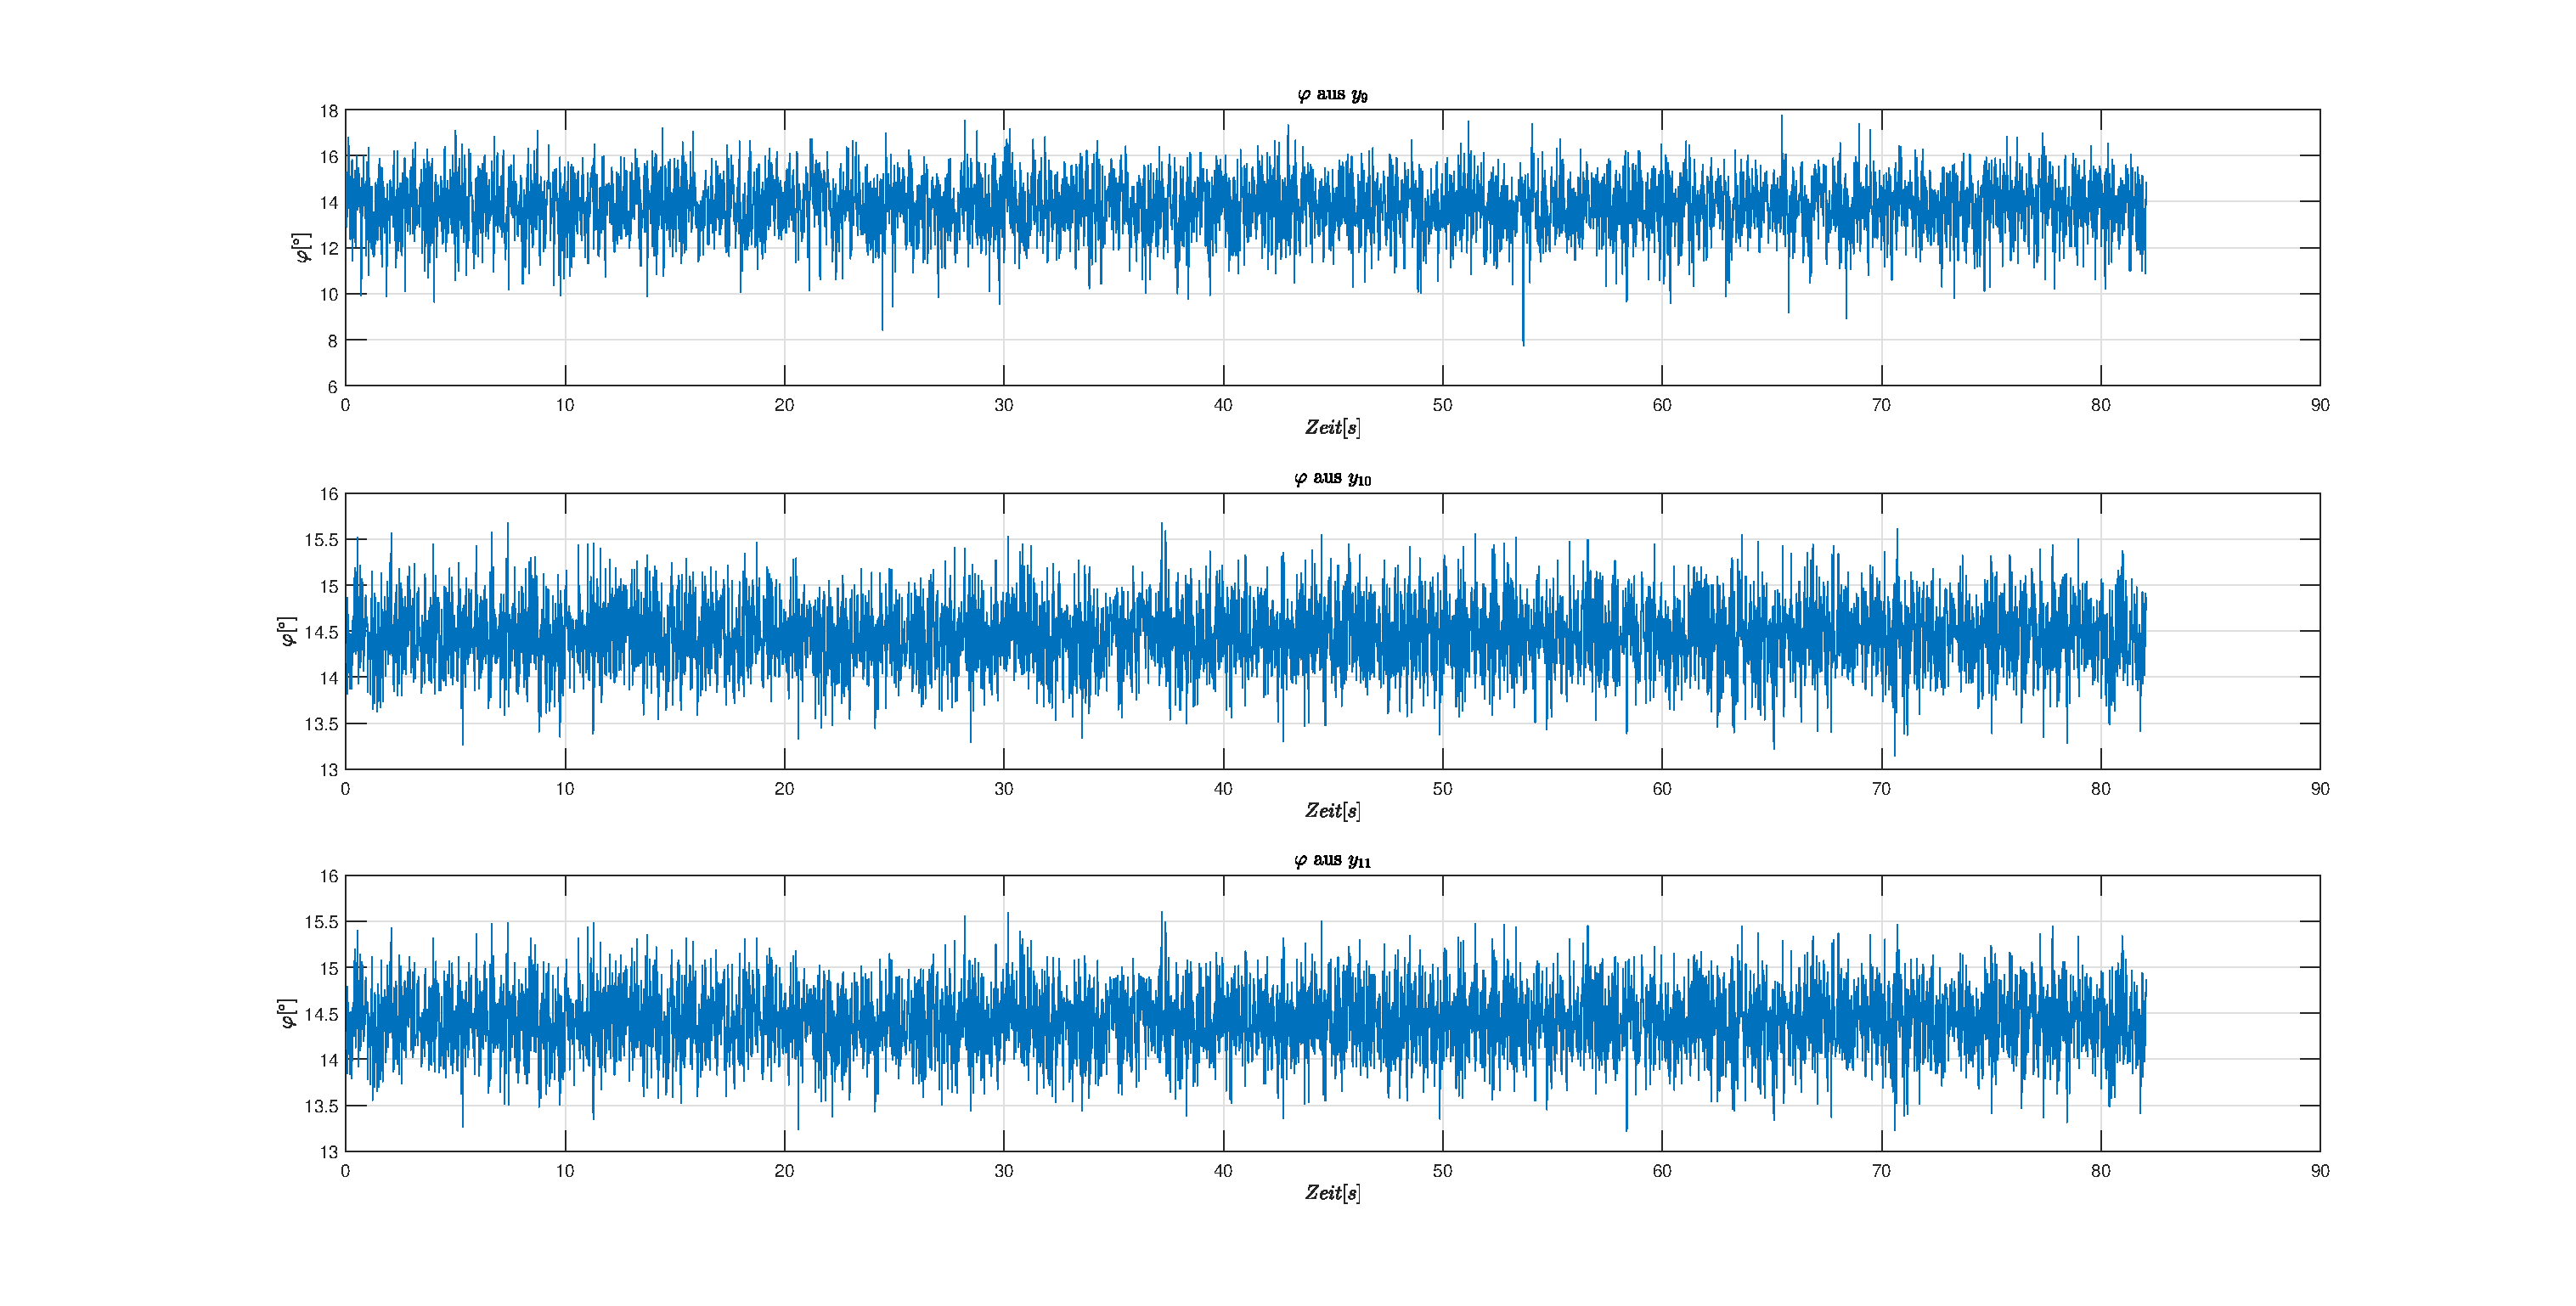
\includegraphics[width=\linewidth]{3_Sensorik/img/snr_phi_plot}
\caption{Signal-Rausch-Verhältnis der $\varphi$-Messsysteme, Quelle: eigene Darstellung}
\end{figure}

Da es sich um einen stationären Prozess handelt, kann angenommen werden, dass der Mittelwert der Signale dem Nutzsignal entspricht. Folglich kann mit Hilfe dieser Annahme das Signal-Rausch-Verhältnis berechnet werden. 

\begin{equation}
SNR(y_9) = 20.57dB \hspace{35pt}  SNR(y_{10}) = 31.21dB \hspace{35pt} SNR(y_{11})=31.50dB
\end{equation}

\subsubsection{Diskrete Fourier-Transformation (DFT)}
Die Beurteilung der dynamischen Störungen erfolgt über eine Spektralanalyse. Hierfür wird die DFT der Messgrößen berechnet. Um die Interpretation der DFT-Spektren zu ermöglichen, wird zuerst der Zusammenhang der DFT und der Fourier-Transformation des zu Grunde liegendem Signal hergeleitet.
Die Fourier-Transformation basiert auf der Theorie, dass alle zeitkontinuierlichen Signale aus einer Summe von harmonischen Schwingungen synthetisiert werden können. Der Betrag der Fourier-Transformation gibt die Amplituden der beteiligten Schwingungen wieder. Nun ergibt sich die Frage wie das Spektrum eines zeitdiskreten Signals, das über einen begrenzten Zeitraum abgetastet wird, berechnet werden kann. Hierfür wird zunächst die komplexe harmonische Schwingung $x_n$ mit der Frequenz $f$ betrachtet, welche mit einer Frequenz $f_a$ ($T_a=1/f_a$) abgetastet wird. Mit Hilfe der normierten Kreisfrequenz $\Omega=2\cdot \pi \cdot f/f_a$, welche das Verhältnis der Schwingungsfrequenz und der Abtastrate darstellt, ergibt sich die folgende Funktion für $x_n$.

\begin{equation}
x_n = e^{j\cdot 2 \cdot \pi \cdot  n \cdot \frac{f}{f_a}} = e^{j\cdot n\cdot \Omega}
\end{equation} 

Wenn nun ein System, welches die diskrete Impulsantwort $h_n$ besitzt, von dem Signal $x_n$ angeregt wird, ergibt sich der folgende Zusammenhang für dessen Ausgangssignal $y_n$.

\begin{equation}
y_n = h_n * x_n = \sum^{\infty}_{k=-\infty}h_k \cdot e^{j\cdot\Omega\cdot(n-k)} = e^{j\cdot n\cdot \Omega} \cdot \sum^{\infty}_{k=-\infty} h_k \cdot e^{-j\cdot \Omega \cdot k}
\end{equation}

Hieraus folgt, dass die Antwort eines Systems auf eine diskrete harmonische Schwingung als Produkt der Schwingung mit dem Term $\sum h_k \cdot e^{-j\cdot \Omega \cdot k}$. Dieser kann somit als Systemverstärkung einer komplexen Eingangsschwingung mit der normierten Frequenz $\Omega$ interpretiert werden. Diese Systemeigenschaft entspricht der Aussage der gewöhnlichen Fourier-Transformierten einer zeitkontinuierlichen Übertagungsfunktion. Deshalb gilt für die DTFT (Discrete-Time-Fourier-Transform) eines Signals $x_n$:
\begin{equation}
X_{DTFT}(\Omega) = \sum^{\infty}_{k=-\infty} x_k \cdot e^{-j\cdot \Omega \cdot k}
\end{equation}
Hierbei ist zu beachten, dass die DTFT lediglich in Abhängikeit der normierten Kreisfrequenz $\Omega$ berechnet werden kann. Dies ist eine Folge der Abtastung, da das zeitdiskrete Signal $x_n$ keine Information üben den zeitlichen Abstand seiner Stützstellen enthält. Somit können auch die absoluten Frequenzen des Spektrums nur mit Hilfe der Abtastrate $f_a$ rekonstruiert werden. Für den Zusammenhang zwischen dem FT-Spektrum $X(j\omega)$ des ursprünglichen, zeitkontinuierlichen Signal  und dem DTFT-Spektrum $X_DTFT(\Omega)$ des zeitdiskreten Signales :
\begin{equation}
\frac{1}{f_a}X_{DTFT}(\frac{\omega}{f_a}) = X(j\omega)
\end{equation}

Die Problematik der DTFT liegt darin, das es sich zwar um ein zeitdiskretes Signal handelt, dieses aber nach wie vor über einen unendlichen Wertebereich definiert ist. D.h. es liegt eine geschlossene Funktion vor. Somit ermöglicht die DTFT nicht die Berechnung der Spektralanteile eines Signales, wessen Abtastwerte nur über einen begrenzten Zeitraum bekannt ist. Zusätzlich ist die DTFT selbst eine kontinuierliche Funktion und somit nur schwierig auf digitalen Rechnern umsetzbar. Deshalb soll nun erläutert werden wie ein diskretes Spektrum eines abgetasteten Signals, welches nur über einen begrenzten Zeitraum definiert ist, berechnet werden kann. Hierfür wird das Signal $\hat{x}_n$ betrachtet, welches für die ersten $N$ Abtastwerte der komplexen harmonischen Schwingung $x_n$ entspricht und anschließend verschwindet.
\begin{equation}
\hat{x}_n = \begin{cases}
				x_n & n \in [0;N-1] \\
				0   & n \not\in [0;N-1]
				\end{cases}
\end{equation}
Somit ergibt sich für die DTFT von $\hat{x}_n$:
\begin{equation}
\hat{X}_{DTFT}(\Omega) = \sum^{\infty}_{k=-\infty}\hat{x}_k \cdot e^{-j\cdot k \cdot \Omega} = \sum^{N-1}_k=0 x_k \cdot e^{-j \cdot k \cdot \Omega}
\end{equation}
Wird nun die DTFT wiederum über $N$ Werte diskretisiert erhält man als Ergebnisse die diskrete Fourier-Transformation (DFT).
\begin{equation}
X_{DFT}(m) = \sum^{N-1}_{k=0} x_k \cdot e^{-j\cdot k \cdot \Omega_m} \hspace{35pt} \Omega_m = \frac{2\cdot \pi \cdot m}{N}
\end{equation}
Bei der Herleitung der DFT wird ersichtlich, dass das berechnete Spektrum nicht dem des zeitdiskreten Signales $x_n$ entspricht, sonderm dem Spektrum von $x_n$ multipliziert mit einem Rechteckimpuls, wessen Breite dem Beobachtungszeitraum entspricht. Die Auswirkungen dieser Fensterung auf das DFT-Spektrum werden als Leakage-Effekte bezeichnet. Da für gewöhnlich Informationen über das Spektrum des ursprünglichen, zeitkontinuerlichen Signals gesucht sind müssen einerseits die Leakage-Effekte minimiert werden und der Zusammenhang zwischen FT-Spektrum und DFT-Spektrum hergestellt werden. Falls ein periodisches Signal $x(t)$ wird über einen Zeitraum $T$ beobachtet wird und $T$ kein Vielfaches der Periodenlänge des Signales ist so entstehen Signalsprünge am Ende der Beobachtung. Diese Sprüngen führen zu spektrale Überlappungen, welche wiederum das DFT-Spektrum verfälschen. Deshalb ist der Beobachtungszeitraum mit der Schwingung eines periodischen Signales zu synchronisieren. Des weiteren können Leakage-Effekte minimiert werden indem ein möglichst großer Beobachtungszeitraum gewählt wird. Ist dies der Fall gilt folgender Zusammenahng für Spektralanteile, welche keinen unendlichen Wert besitzen.
\begin{equation}
X_{DFT}(m) \approx f_a \cdot X(j\cdot m \cdot \Delta \omega) \hspace{35pt} \Delta\omega = 2\cdot \pi \cdot \frac{f_a}{N}
\end{equation}
Falls das Spektrum $X(j\cdot\omega)$ an der Stelle $m\cdot \Delta \omega$ einen Dirac-Impuls-Anteil besitzt so gilt für den komplexen Fourierkoeffizienten $c_k$ des Signales an dieser Frequenz:
\begin{equation}
X_{DFT}(m) = N \cdot c_k
\end{equation}